\chapter{Utilizzo di un opamp}

\section*{Obiettivo}

Testare i vari amplificatori operazionali e analizzare la loro risposta in frequenza.

\section*{Svolgimento}
\subsection*{OP37\footnote{\href{https://www.analog.com/media/en/technical-documentation/data-sheets/OP37.pdf}{Datasheet OP37}}}
%%TODO aggiungere cose vecchie


L'opamp OP37 è stabile con un guadagno >= 5. 
Alimentiamo l'opamp con una tensione VCC = +10V e VEE = -10V.


Proviamo ad impostare, usando l'opamp in configurazione non invertente, un guadagno inferiore a 5 per vedere come si comporta.

\begin{figure}[H]
\centering
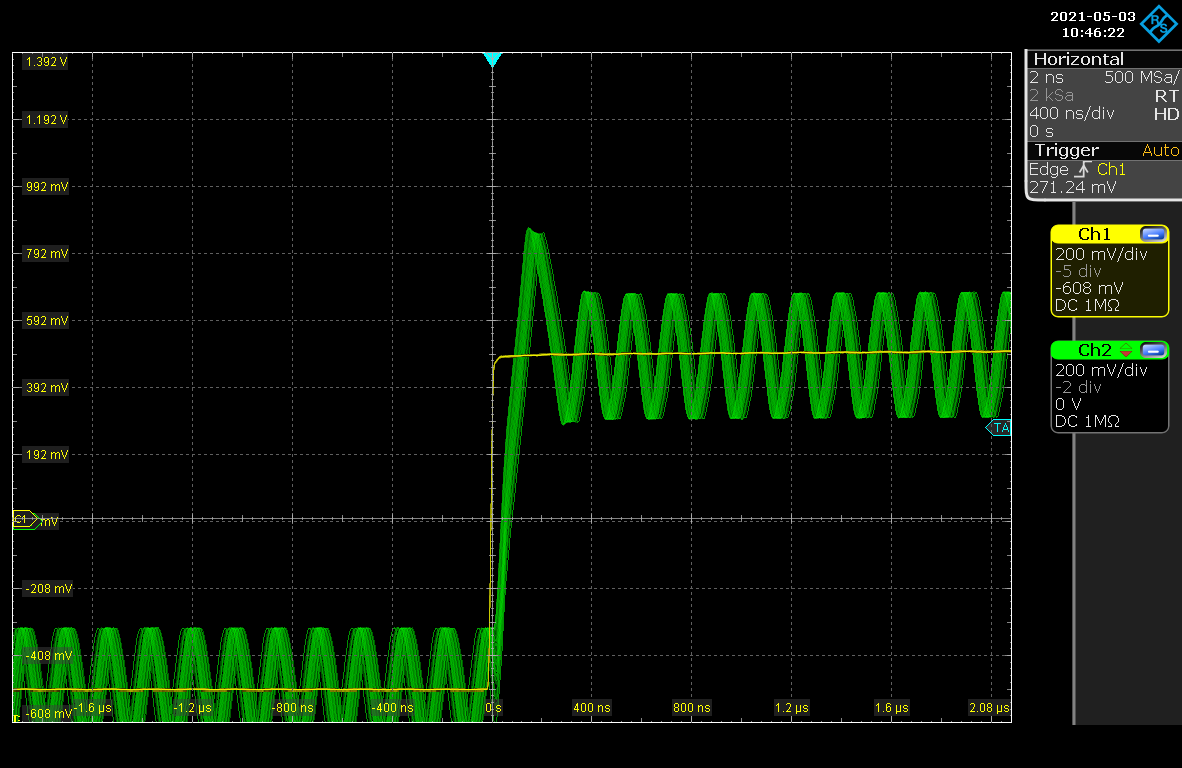
\includegraphics[width=0.75\textwidth]{assets/exp8/Guadagno_1.png}
\caption{Configurazione con gain pari a 1}
\end{figure}

\begin{figure}[H]
\centering
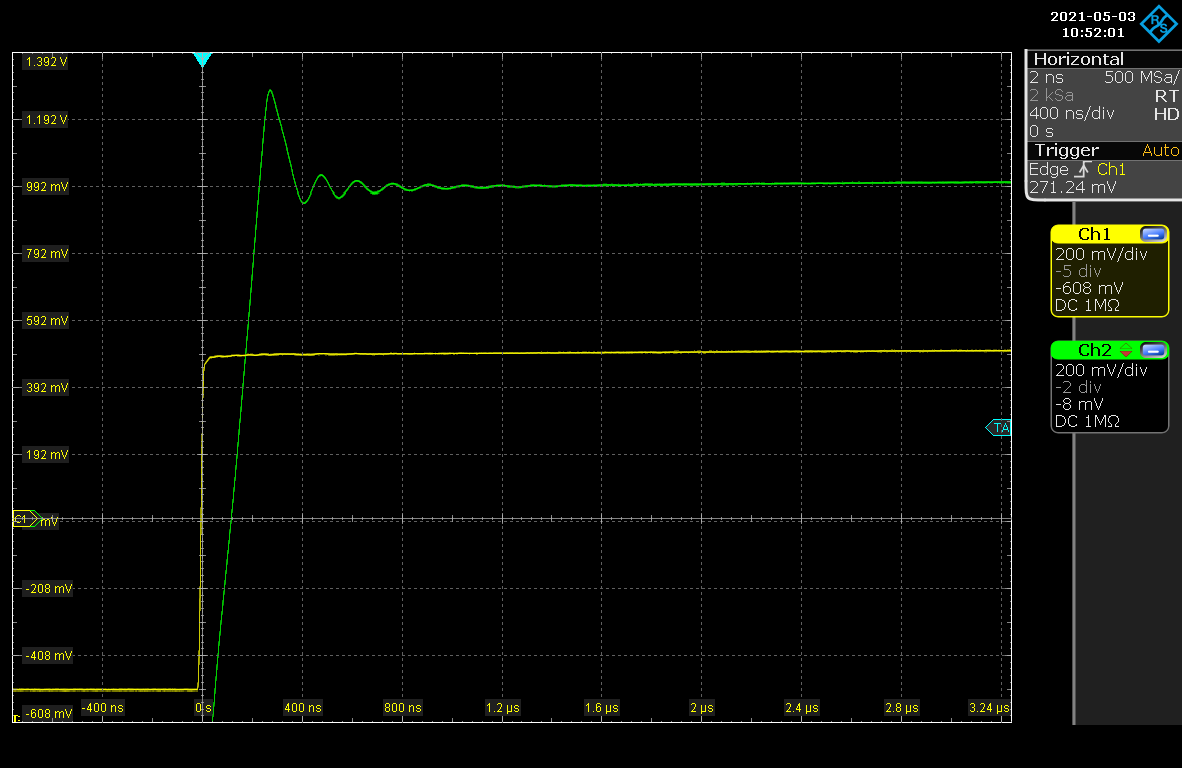
\includegraphics[width=0.75\textwidth]{assets/exp8/Guadagno_2.png}
\caption{Configurazione con gain pari a 2}
\end{figure}

Andiamo ad osservare la risposta al gradino e notiamo che il sistema oscilla: nel primo caso oscilla all'infinito senza convergere, nel secondo caso il sistema oscilla ma alla fine converge.

Proviamo quindi ad impostare un guadagno superiore a 5.

\begin{figure}[H]
\centering
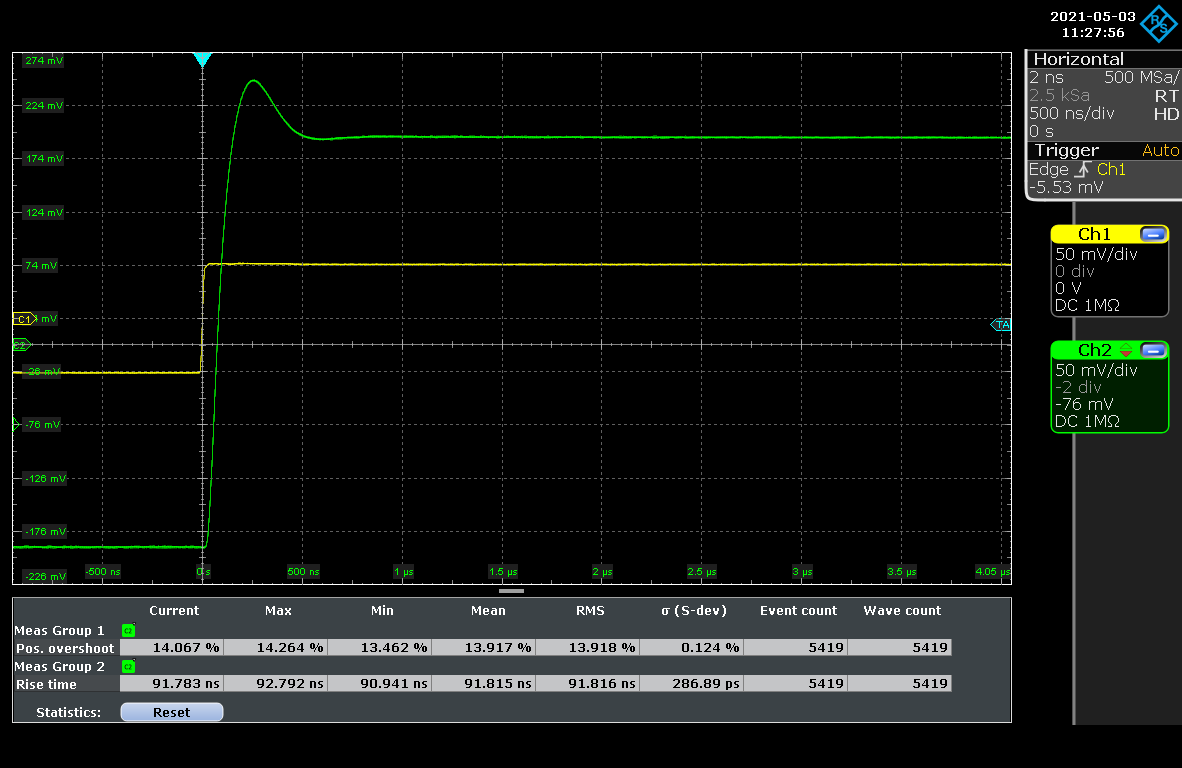
\includegraphics[width=\textwidth]{assets/exp8/Guadagno_7.6666_pt2.png}
\caption{Configurazione con gain pari a $7.\overline{6}$}
\end{figure}

Provando sempre la risposta al gradino notiamo che il sistema non oscilla più. Tuttavia è presente un overshoot, ovvero una sovraelongazione rispetto al valore voluto.
Sfruttando le funzioni di misura dell'oscilloscopio possiamo andare a vedere quanto è in percentuale rispetto al valore voluto.
Come mostrato in figura l'overshoot è circa del $14\%$, un risultato comunque accettabile.

\vspace*{0.5cm}

\noindent
Andiamo poi a testare l'opamp usando una configurazione invertente.

Partiamo impostando un guadagno inferiore a 5.
\begin{figure}[H]
\centering
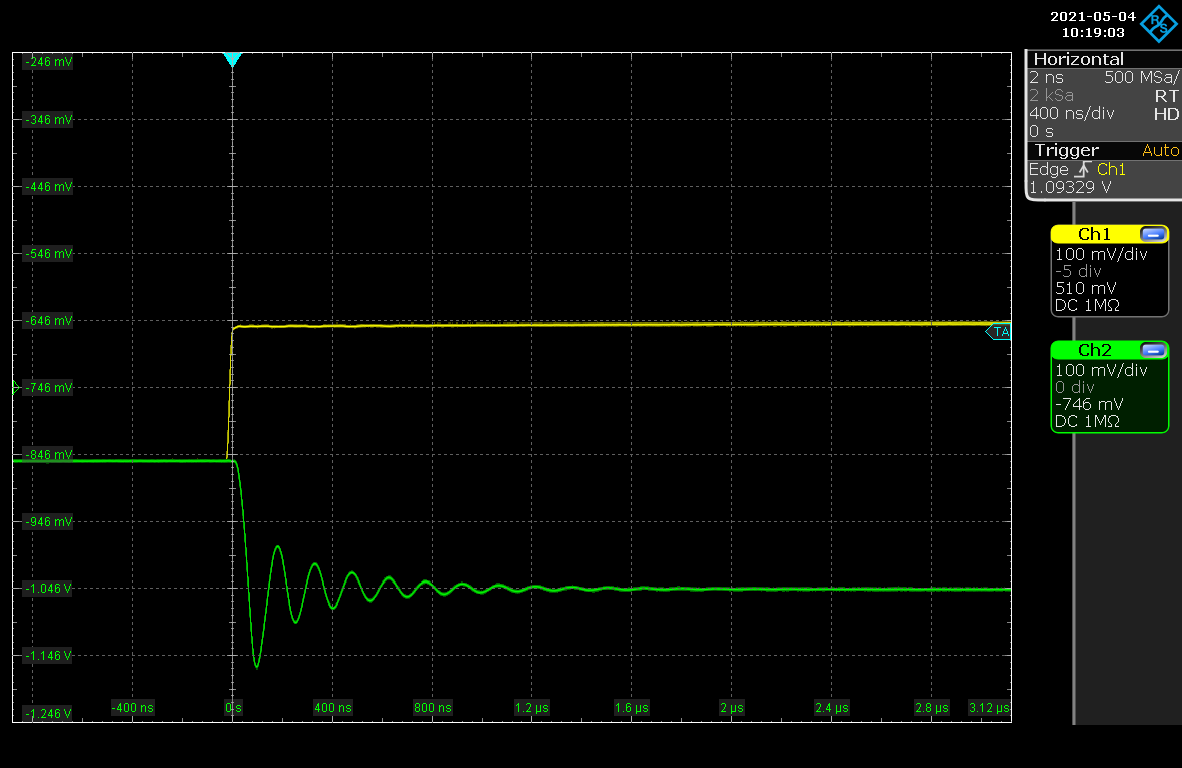
\includegraphics[width=0.7\textwidth]{assets/exp8/invertente_guadagno_1.png}
\caption{Configurazione invertente con guadagno 1}
\end{figure}

Anche in questo caso, come ci aspettavamo, notiamo un comportamento oscillatorio del sistema.

\begin{figure}[H]
\centering
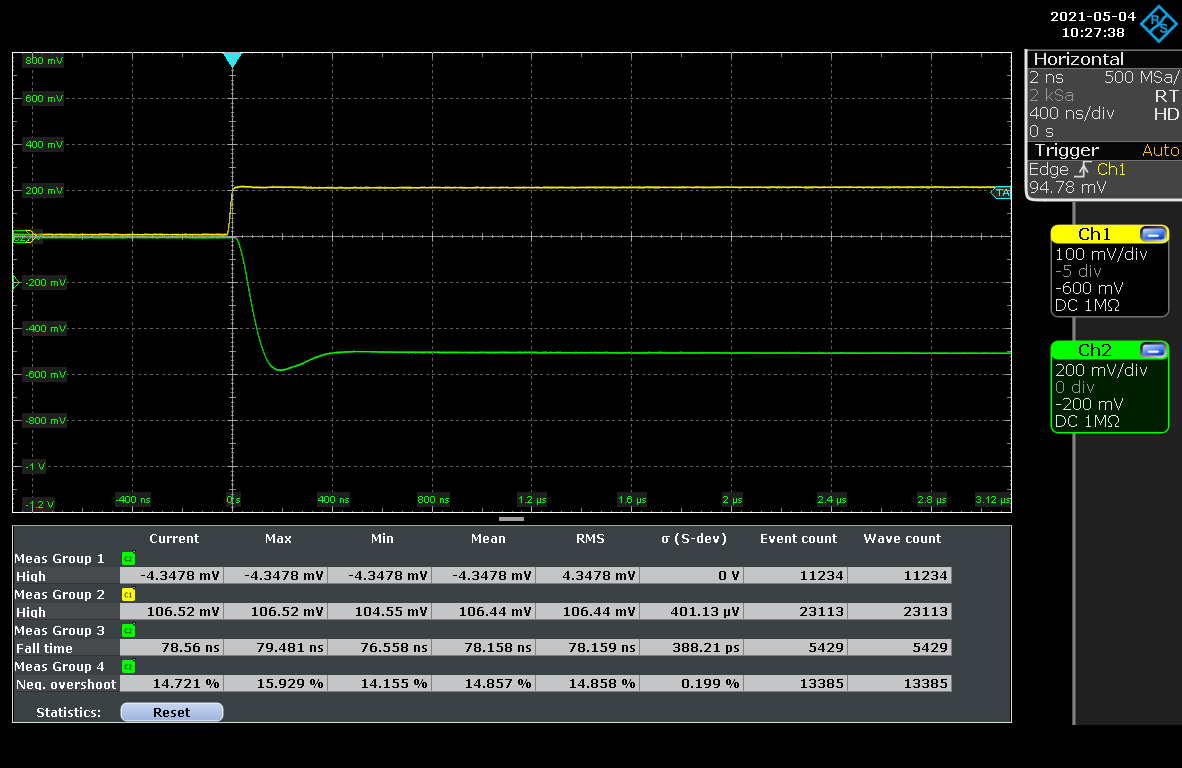
\includegraphics[width=0.7\textwidth]{assets/exp8/invertente.png}
\caption{Configurazione invertente}
\end{figure}

Andiamo ad aumentare il guadagno: in questo modo il sistema non oscilla più. Anche in questo caso notiamo un piccolo overshoot.

Possiamo poi andare a vedere come il guadagno dell'opamp sia dipendente dalla frequenza del segnale in ingresso.
Proviamo ad impostare con il generatore di funzioni una sinusoide con frequenza via via maggiore (da 1MHz a 10Hz).

\begin{figure}[H]
\centering
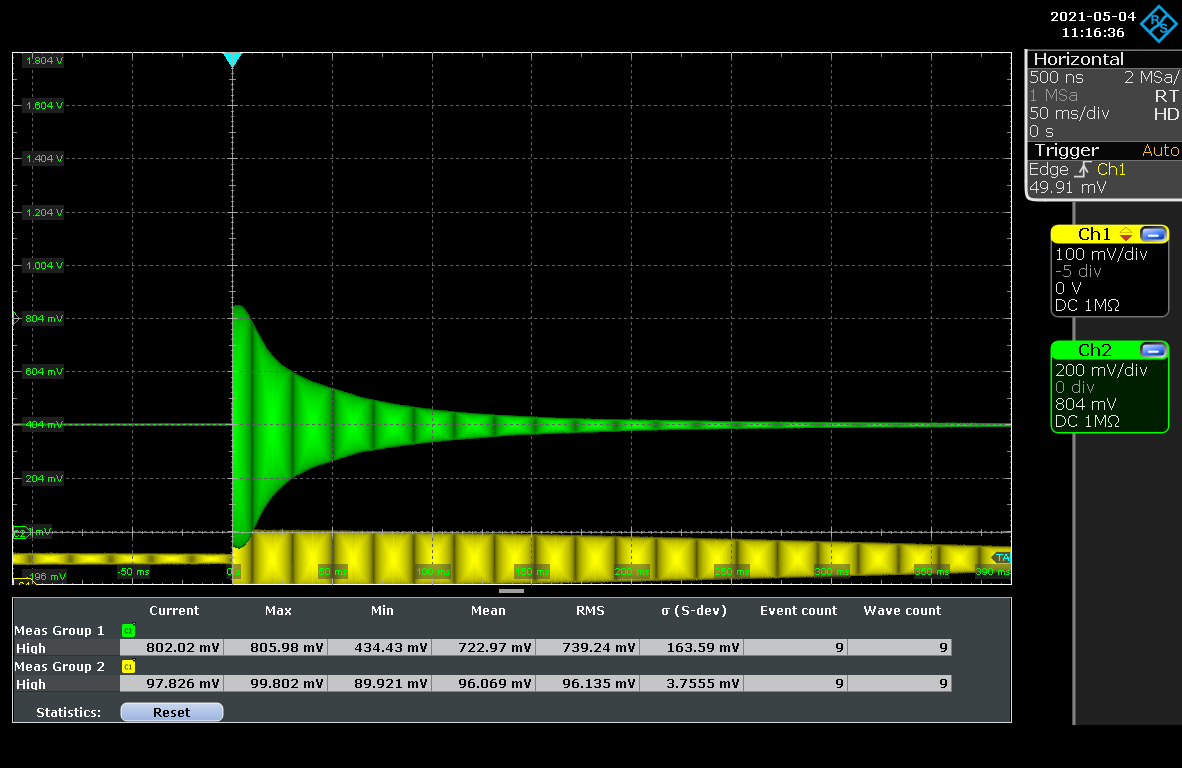
\includegraphics[width=\textwidth]{assets/exp8/Screenshot_2021-05-04_1_111636.png}
\caption{Andamento del guadagno in base alla frequenza}
\end{figure}
Notiamo come il gain diminuisca all'aumentare della frequenza del segnale in ingresso.

\newpage
\subsection*{AD9631\footnote{\href{https://www.analog.com/media/en/technical-documentation/data-sheets/AD9631_9632.pdf}{Datasheet AD9631}}}

Andiamo poi a testare un altro opamp più veloce e con guadagno minimo 1: l'opamp AD9631. Alimentiamo questo opamp con VCC 5V e VEE -5V.

Per l'esperimento sono stati usati i seguenti componenti e parametri:

\begin{itemize}
    \item OPAMP AD9631, configurazione non invertente
    \begin{itemize}
        \item R1: 910 ohm
        \item R2: 110 ohm
        \item Gain: 9.27
    \end{itemize}
    
    \item Funzione generata:
    \begin{itemize}
        \item Onda quadra a 1khz
        \item Amplitude: 102mV
        \item High: 103mV
    \end{itemize}
    
\end{itemize}

La bandwidth indicata dal datasheet (320MHz) è valida per il guadagno 1, avendo impostato guadagno 9.27 abbiamo che la bandwidth sarà

\begin{displaymath}
BW_{guadagno} = \frac{BW}{guadagno} = \frac{320 \si{MHz}}{9.27} \approx 34.5 \si{MHz}
\end{displaymath}

Misuriamo il tempo di rise dell'opamp AD9631. Per rise time intendiamo il tempo che impiega il segnale per passare dal $10\%$ dell'ampiezza al $90\%$.
Per fare un'analisi più accurata dobbiamo prendere in considerazione anche il tempo di salita della funzione generata, sfruttando la seguente formula:

\begin{displaymath}
 tRise = \sqrt{tRiseOpAmpMisurato^2 - tRiseFunctGen^2} = \sqrt{43,903^2 - 15,862^2} \approx 40.93 \si{ns}
\end{displaymath}

Quindi nel nostro caso il tempo di rise è 40.93 nanosecondi.

Un parametro fondamentale degli opamp è la bandwidth, definita come la frequenza a cui l'ampiezza del segnale è al $70\%$ della flat response, ovvero quando siamo alla frequenza corrispondente a $-3 \si{dB}$.

Sappiamo che esiste una relazione tra bandwith e rise time data dalla seguente equazione:
\begin{displaymath}
tRise = \frac{0.35}{BW}
\end{displaymath}
Da qui ricaviamo che:
\begin{displaymath}
BW = \frac{0.35}{tRise}
\end{displaymath}
Quindi possiamo ricavare la bandwidth del nostro amplificatore:
\begin{displaymath}
BW = \frac{0.35}{40.93\si{ns}} \approx 8.45 \si{MHz}
\end{displaymath}

Notiamo un forte scostamento tra la bandwidth da noi calcolata, e la bandwidth teorica.

Innanzitutto notiamo come, guardando le curve sui diagrammi di Bode, la bandwidth indicata nella prima pagina del datasheet sia raggiungibile soltanto in condizioni specifiche.
La bandwidth dipende anche dalla resistenza di feedback, dal carico a cui è collegata l'uscita dell'opamp, dal guadagno impostato, dall'ampiezza del segnale in ingresso etc \dots

\begin{figure}[H]
\centering
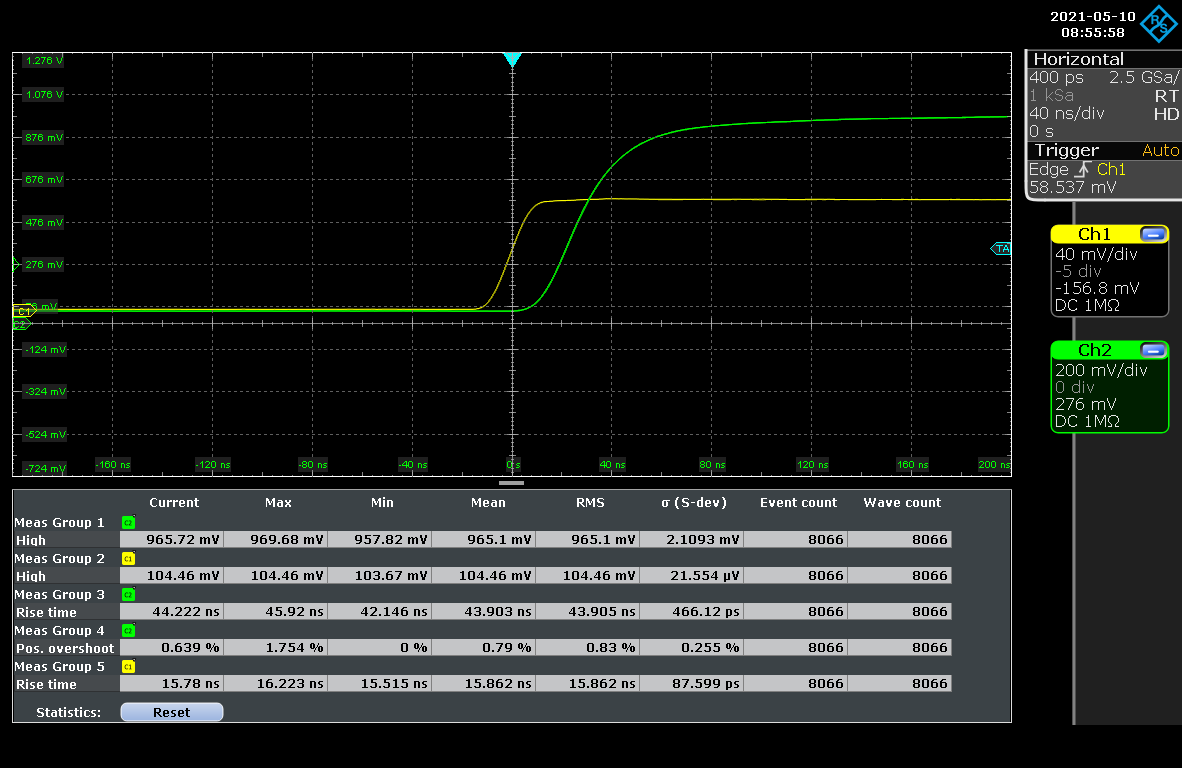
\includegraphics[width=\textwidth]{assets/exp8/Screenshot_2021-05-10_0_085558.png}
\caption{Esperimento per il rise time}
\end{figure}





